\chapter{Reactor Design Verification}
    As discussed earlier, the scope of this project was not to develop a mature
reactor concept. Most of this work focused on modeling the mass of the
reactor as a function of flow inputs and thermal power requirements. It is
prudent however, to verify that the chosen reactor design is feasible as a
reactor concept. The purpose of this section is to convince the reader that
the chosen reactor design is valid, and with significant engineering effort,
could be developed into a working nuclear reactor. To this end, more detailed
neutronics modeling was performed on the chosen reactor design.

\section{Homogeneous Approximation}
All MCNP modeling was performed based on a homogeneous approximation for core
materials. The fuel, coolant, and cladding compositions were smeared to form a
single homogeneous core region. This approximation simplified the geometry which
helped automate the generation of thousands of input files for parametric
sweeps. A homogenous fuel mixture was deemed appropriate because there is little
moderation in the modeled systems. Average neutron energies are higher in the
absence of a moderator and higher energy neutrons have large mean free paths in
matter. This increased mean free path reduces the importance of small geometric
features.

The homogeneous approximation is known to be acceptable from decades of
experience modeling fast nuclear reactors. Still, it is important to check
assumptions. The homogeneous approximation was checked by comparing a
heterogeneous and a homogeneous \keff result for the same \uran mass and core
geometry. Coolant channels were added to the heterogeneous model and the fuel
fraction of the homogenous model was adjusted to match the hetergeneous fuel
fraction. Table \ref{tab:homog_validate_params} shows the parameters used for
the validation case. The fuel fraction was chosen to match the fuel fraction
caused by 54 coolant channels in the heterogeneous model.

\begin{table}[h]
  \centering
  \caption{Parameters for validating homogeneous geometry approximation}
  \begin{tabular}{ll}
    \toprule
     Core Radius                		   & 16 [cm] \\
     Fuel Enrichment 					   & 93\% $^{235}$U [-]\\
     Reflector Thickness				   & 15 [cm]\\
     Coolant Channel Radius                & 0.5 [cm] \\
     Cladding Thickness                    & 0.031 [cm] \\
     Fuel Fraction                         & 0.9405 [-]\\
     Core Aspect Ratio					   & 1 [-] \\
     Fuel Temp  						   & 300 [K]\\
     Reactor Physics Code, Data			   & MCNP6.1, ENDF-7.2
  \end{tabular}
  \label{tab:homog_validate_params}
\end{table}

The heterogeneous geometry is shown in Figure \ref{fig:hetero_xy}. Both models
were run with 290 active cycles and 100,000 histories per cycle to ensure
solution convergence. Table \ref{tab:homog_validate_results} shows the results
of the validation. The results are in good agreement.

\begin{figure}[h]
    \centering
    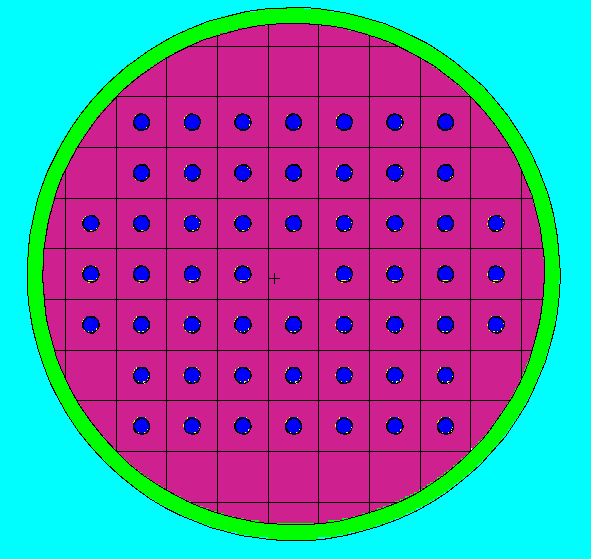
\includegraphics[width=3in]{../images/hetero_xy.png}
\caption{Heterogeneous reactor model for validating homogeneous geometry
approximations}
\label{fig:hetero_xy}
\end{figure}


\begin{table}[h]
  \centering
  \caption{Results of homogeneous geometry validation}
  \begin{tabular}{lll}
    \toprule
     Model                             & \keff & stdv       \\
    \midrule
     Homogeneous              		   & 1.13777 & 0.00013  \\
     Heterogeneous 					   & 1.13159 & 0.00013  \\
  \end{tabular}
  \label{tab:homog_validate_results}
\end{table}

\section{Reactivity Verification}
After the reactor and power cycle was optimized with the total system optimizer,
it was important to verify the resultant reactor design was valid. There was
confidence in the coolability of the design to the extent that the 1D heat
transfer equations accurately model the system. There exists more uncertainty
with the neutronic validity of the reactor.

\onehalfspacing
\begin{enumerate}
    \item The core radii are determined by a 3rd degree fit to data
    \item The data for the fit came from constraining a \keff response described
        by a trilinear interpolation
    \item The trilinear interpolation function was generated using stochastically
        generated \keff data from MCNP
    \item Target excess reactivity was used to model depletion effects
\end{enumerate}
\doublespacing

The reality of the neutronics workflow, is that it was too onerous to propogate
uncertainty in the underlying MCNP results, the trilinear interpolation, and the
fitting function to quantify some understanding of the error in reactor mass. In
order to compensate for this defficiency in error propogation, the results of
the optimization were verified with more traditional reactor physics modeling
techniques.

\subsection{BOL Reactivity Verification}
Beginning of life reactivity was validated to show the surrogate neutronics
modeling techniques work for the target reactivity. The next step was to verify
that target BOL reactivity was chosen appropriately. The optimized mass reactor
from the power cycle optimization was used to verify BOL \keff. Table
\ref{tab:bol_validate} shows the inputs from the power cycle, the optimized
design parameters, and the modeled BOL \keff check. The BOL \keff of the optimized reactor
is in good agreement with the target value. 
The reactor has slightly more excess reactivity (~349 pcm) than the
target reactivity. This gives credibility to the \keff modeling techniques.

\subsection{EOL Reactivity Verification}
End of life reactivity was modeled to check the excess reactivity threshold. The
same MCNP model was used with the addition of the depletion features. The core
was depleted for 10 years at varying time steps to have more time fidelity at
BOL. The core fuel region was divided into 5 annular sections of equal volume to
account for non-uniform radial burnup. Figure \ref{fig:depl_core_xy} shows the
xy view of the model used to verify EOL reactivity.

\begin{figure}[h]
    \centering
    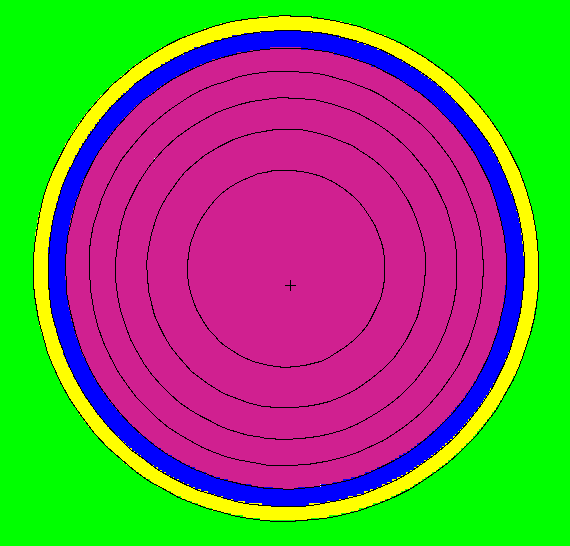
\includegraphics[width=3in]{../images/depl_core_xy.png}
\caption{5 annular core regions to model homogeneous depletion.}
\label{fig:depl_core_xy}
\end{figure}

Table \ref{tab:bol_validate} shows the results of the EOL reactivity
validation. Note, the FOM for EOL reactivty is \keff > 1. Both BOL and EOL
reactivity satisfy neutronics requirements. 

\begin{table}[h]
  \centering
  \caption{Results of homogeneous geometry validation}
  \begin{tabular}{lll}
    \toprule
    Flow Cycle Input                        & Value \\
    \toprule
    T$_{in}$/T$_{out}$ & 793.8/900 [K]\\
    P$_{in}$/P$_{out}$ & 1.79E+04/1.74E+04 [Pa]\\
    Flow Rate & 1.2722 [kg/s]\\
    Thermal Power & 167.80 [kW]\\
    \toprule
    Optimized Design & Result\\
    \toprule
    Core Radius & 12.12 [cm]\\
    Fuel Fraction & 0.74 [-]\\
    Reactor Mass & 123.53 [kg]\\
    BOL \keff & 1.01349 ($\pm$0.00051)
    EOL \keff & 1.00345 ($\pm$0.00049)
  \end{tabular}
  \label{tab:bol_validate}
\end{table}

Figure \ref{fig:dep_curve} shows the reactivity curve over the 10 year mission
life. The blue line shows \keff = 1. The reactor has sufficient reactivity to
remain critical throughout the 10 year mission.

\begin{figure}[h]
    \centering
    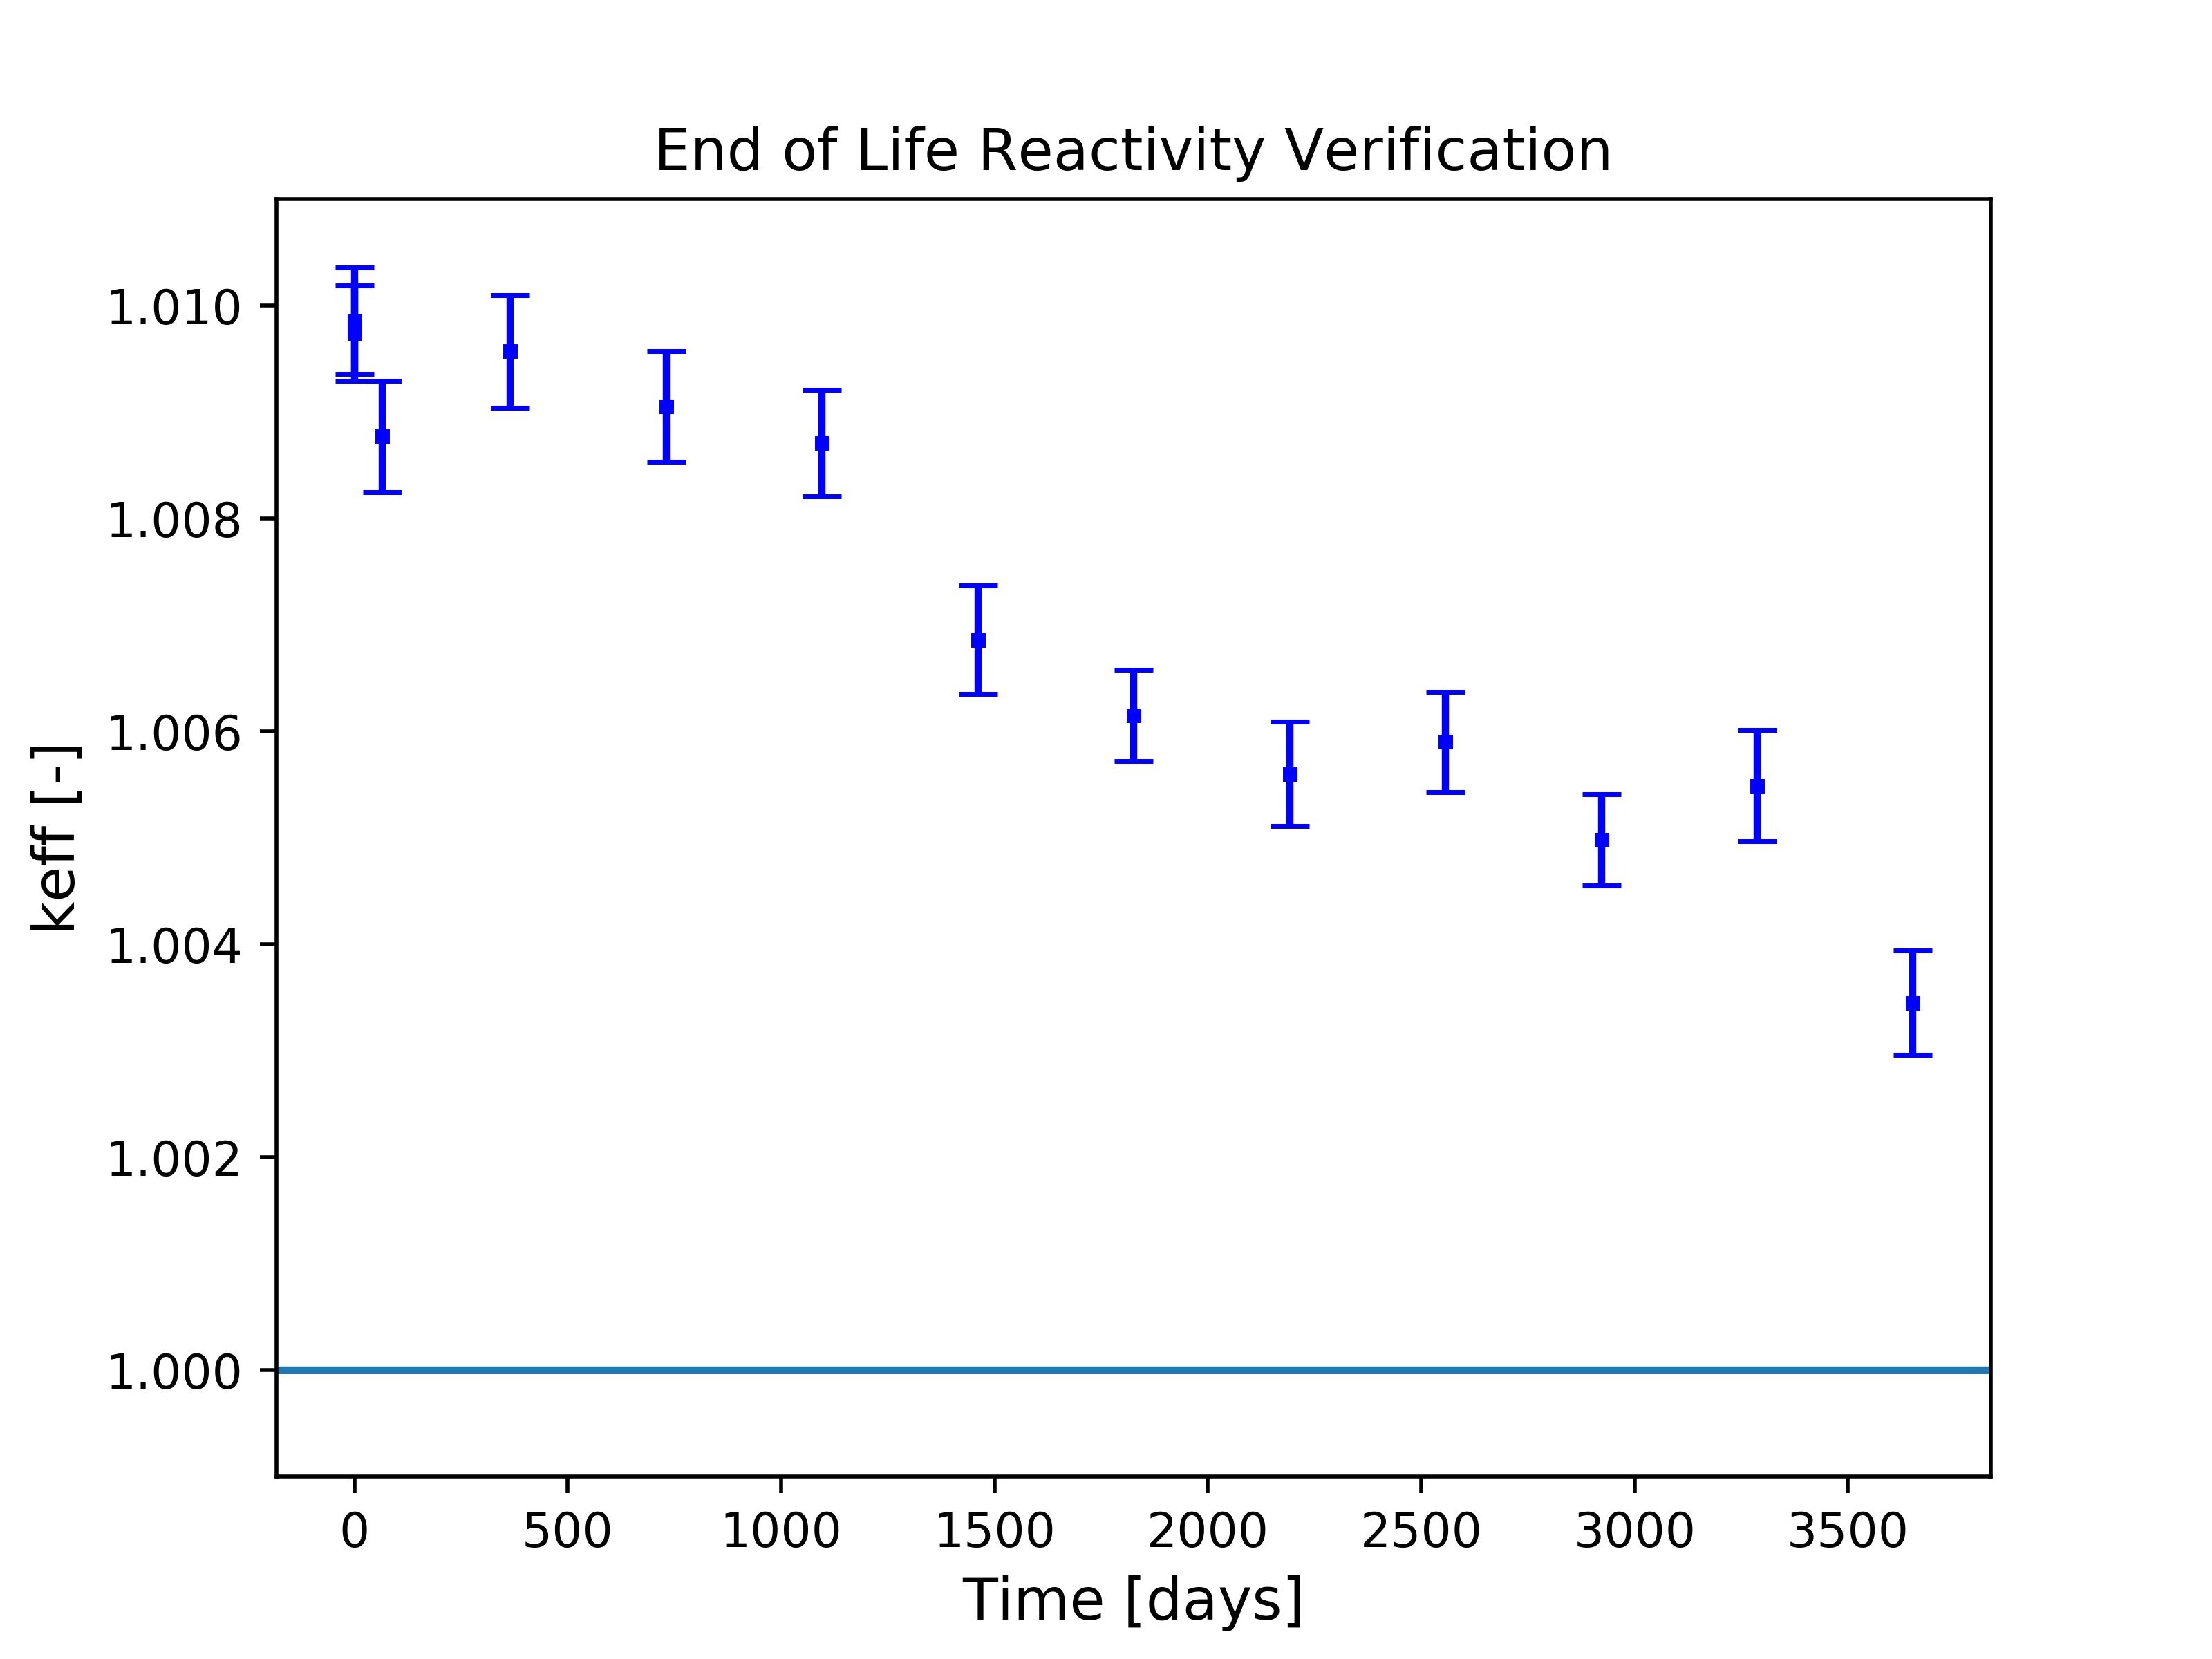
\includegraphics[width=3in]{../images/depletion_results.png}
\caption{10 year reactivity curve.}
\label{fig:depl_curve}
\end{figure}
